\documentclass[10pt,a4paper]{article}
\usepackage[utf8]{inputenc}
\usepackage{amsmath}
\usepackage{amsfonts}
\usepackage{amssymb}
\usepackage{graphicx}
\author{COMPIEGNE MAITE VANROYE VICTORIEN}
\title{GEOLOCALISATION, LES NOUVEAUX OBJETS}
\begin{document}
\paragraph{Introduction}
Ici se trouvera l'introduction
\paragraph{Présentation de l'existant}
De nos jours, il existe des cartes de géolocalisation utilisant un web service qui permet à l'utilisateur de trouver les coordonnées géographiques (latitudes/longitudes) et la vitesse de son véhicule( on utilise un GPS et un Accéléromètre).\\Ils existent déjà des cartes produites par différents fournisseurs avec des tarifs selon le matériel.\\Par exemple la carte traceur geo-302 au prix de 290 euros sans abonnement mais, elle nécessite l'achat d'une carte SIM avec un abonnement. Cette carte à une faible autonomie 7 jours en mode veille.\\Ensuite, il existe le fournisseur Locster avec une gamme de produit et de tarif pour tous types d'utilisateurs. Ici aussi il utilise le réseau des opérateurs GSM.\\L'un des packs les moins chères actuellement est à 299 euros pour un abonnement de deux mois et le boitier d'une taille de taille 8x5x4 cm, 110g et la carte SIM. Après les deux mois d'abonnement l'utilisateur doit payer 9 euros/mois. Son autonomie est de 1 à 5 mois selon l'utilisation. Pour 5 mois on a 1 position/jour et pour 1 mois on a 1 position/par heure).\\L'un des packs les plus chères est à 614 euros pour un abonnement de 24 mois avec là aussi l'équipement (boitier 4x7,9x8,7 cm 333g ) et la carte SIM fournit ensuite l'abonnement passe à 12 euros/mois). Pour l'autonomie c'est équivalent au matériel précédent. 
\paragraph{Sigfox}
est une technologie développé par l'entreprise du même nom. Cette entreprise a fait le parie de miser non pas sur le haut débit mais le bas débit afin de limiter au maximum le coût et la consommation énergétique. Leur but étant de fournir un support de communication accessible à tous pour l'Internet des objets.\\ Le premier point important de cette technologie est la consommation énergétique qui est inférieur au gsm habituel qui comme pour nos téléphones abaissent grandement la durée des batteries. Ici, sur 162305984 Envois Sigfox, on a économisé 4055703 Watt-heure par rapport au GSM (Source: Site Sigfox), le modem consomme 50 micro-watt comparé au 5000 du cellulaire. \\Le second point intéressant est celui de la couverture du réseau qui contrairement au réseau mobile, les antennes SigFox ont une portée bien supérieur et donc facilite le déploiement. Actuellement, le réseau en France n'est pas encore terminé mais le sera prochainement. A l'international, la société a fait une levé de fond pour commencer le déploiement, vous pourrez observer l'avancement sur le site de Sigfox de celui-ci. La grande contrainte actuellement de cette technologie est qu'elle n'est disponible qu'en émission, les modem peuvent envoyer mais pas encore recevoir. L'entreprise Sigfox attend la fin de déploiement du réseau pour mettre en place cette fonctionnalité ce qui viendra compléter parfaitement les capacités.\\Troisième points qui est la contrainte majeur est la taille des messages et le débit qui est de 12 Octets/Messages à 100 Bits/Secondes et de 140 Messages/Jours. Mais cette limitation s'explique par le cadre d'utilisation visé, les objets connectés sont très souvent très spécialisé et sont limité dans leur fonctionnalité, on peut donc voir que leur besoin en débit est très faible, sauf cas de caméra ou d'autre capteur gourmand en donnée, si on prend pour exemple un capteur de température et humidité, il est très facile de faire passer dans les messages ces données et même le niveau de batterie. Et là, encore l'Internet des objets n'est pas idées qui manquent et Sigfox apparait comme l'un des meilleurs outils pour la communication de ceux-ci. Nous allons voir maintenant comment nous avons mis en place cette technologie dans le cadre de carde de localisation.
\paragraph{Présentation des deux design de carte}
Pour la réalisation de ce projet nous avions une contrainte au niveau de la taille de la carte, celle-ci ne devais pas être trop grande pour pouvoir être intégré dans un bus ou sur des vêtements.\\
Pour commencer nous avons réalisé la carte avec un TD1208, un GPS, un accéléromètre et un Pic.
Mais pour un gain de place nous avons recherché différentes méthodes pour réduire la taille de la carte. Nous avons donc choisi de changer le TD1208 en un TD1204.\\ 
 Pour vérifier quelle méthode est la mieux adaptée notre projet nous avons réalisé les deux cartes, l'un avec le TD1208 et l'autre avec un TD1204\\ Voici les deux cartes permettant de réaliser un traceur GPS. \\Carte avec le TD1204 avec ses avantages et ses inconvénients. \\Les avantages : \\Grâce au TD1204 programmable et qui regroupe en un seul composant le GPS, l'accéléromètre et un TD1208 il est possible de supprimer plusieurs composants de la carte (GPS, Accéléromètre, pic,…). Malgré la taille plus grande de ce composant il nous permet de gagner de la place, mais aussi de supprimer des contraintes liée aux composants tels que le GPS qui nécessite de percer la plaque pour permettre la transmission de l'antenne. \\Ensuite, comme nous avons supprimé plusieurs composants le routage devient simple. Il suffit d'une carte avec deux couches pour respecter la contrainte de taille demandée par le cahier des charges. Ainsi notre carte est  ''propre'', on minimise les grandes pistes qui traversent toute la carte ce qui évite la perte de puissance dans les pistes.\\Les inconvénients :\\Ce composant est assez récent donc sa pérennité n'est pas assurée dans le temps.  
Carte avec le TD1204 avec ses avantages et ses inconvénients. \\Les avantages :\\Ce composant est l'un des produits de Télécom Design qui est produit depuis quelques temps. On est donc sûr que pendant encore quelques temps ce composant sera encore produits.\\ Les contraintes :\\Comme le TD1208 ne regroupe pas plusieurs composants il faut ajouter un GPS, un Accéléromètre un Pic pour le programmé.  Et il faut aussi respecter la spécificité de celui-ci qui nécessite, comme pour le GPS, de percer la plaque. Donc lors du routage on ne peut passer aucune pistes sous ces composants. Ce qui nous oblige à passer sur une carte avec quatre couches et de grandes pistes qui traversent toute la carte, voir même qui passe par les quatre couches pour pouvoir connecté tous les composants. \\Nous avons donc réalisé ces deux cartes aux cours de notre projet donc voici les vues 3D simulé grâce au logiciel Proteus. \\
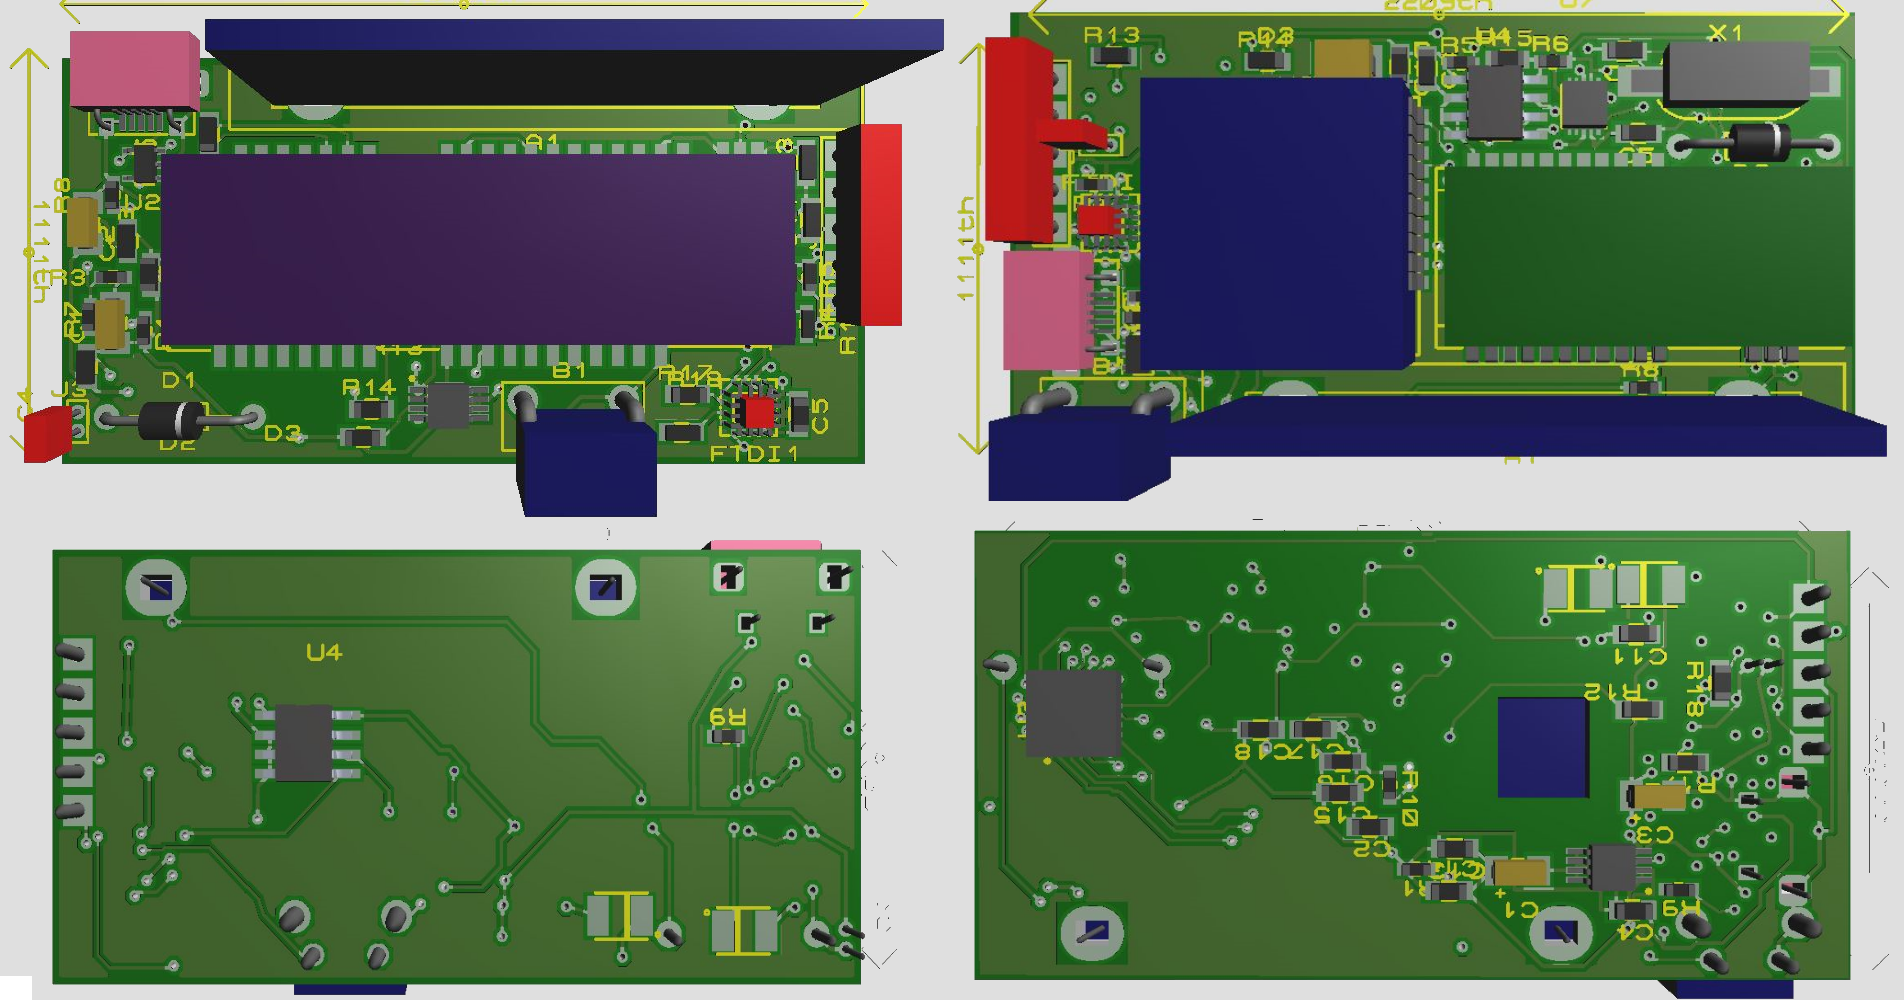
\includegraphics[scale=0.2]{TP1204-1208.png} 

Le TD1208 est en vert le TD1204 est en mauve. 


\paragraph{Bilan de consommation des deux designs + une carte existante}

\end{document}